%%%%%%%%%%%%%%%%%%%%%%
\section{Results}
%
%%%%%%%%%%%%%%%%%%%%%%

\begin{figure}[ht]
\begin{center}
\centerline{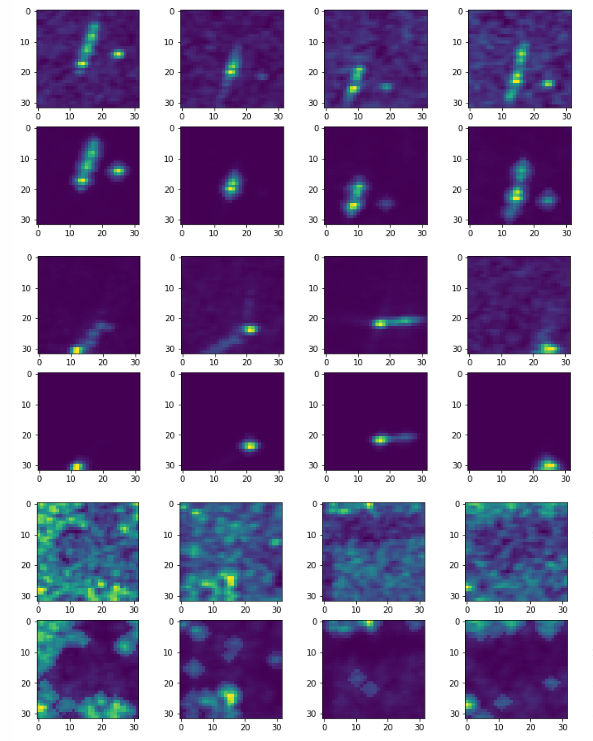
\includegraphics[width=\columnwidth]{images/denoise-final.png}}
\caption{A comparison between noise reduction showing windmills, boats and land based imagery.}
\label{noise-reduction-results}
\end{center}
\end{figure}

\subsection{Filtering clustered objects}

Since clustering is an expensive operation and greatly depends on the distribution of points we first filter our set of result points to remove densely packed zones. We do this by saving all coordinates containing a windmill/boat in a map and checking for each point we add if it has any neighbors, if so it will skip adding this point. By using a map this algorithm has a logarithmic complexity making it feasible to parse large zones like the North Sea. An comparison of how windows don't overlap can be seen in Figure \ref{detection-filtering}.

\begin{figure}[ht]
\begin{center}
\centerline{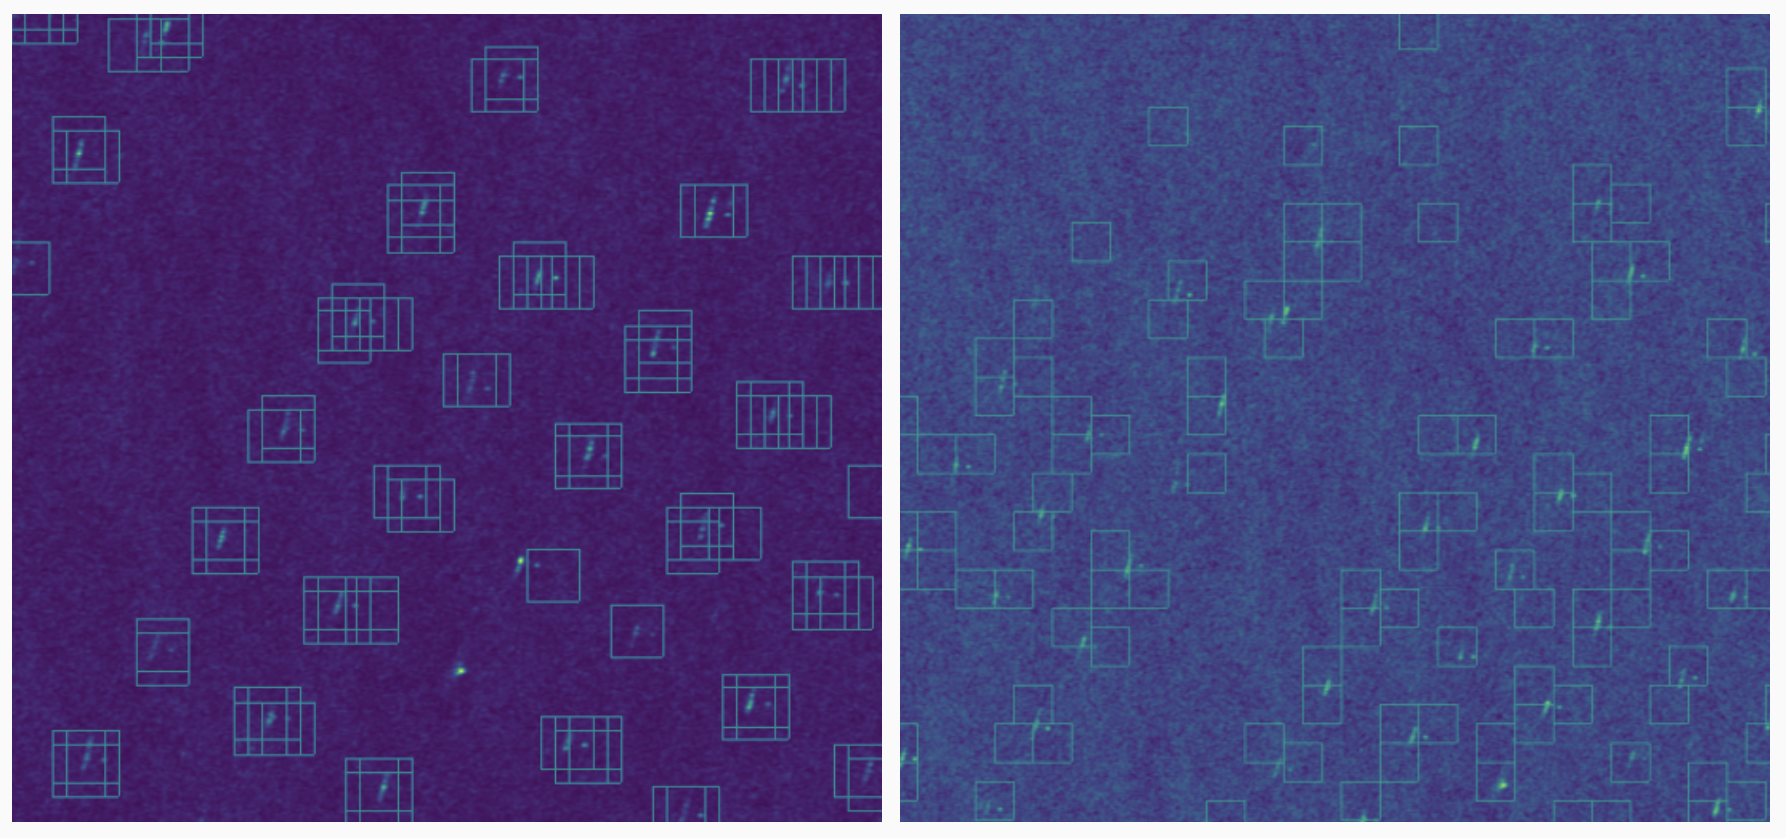
\includegraphics[width=\columnwidth]{images/detection-filtering.png}}
\caption{Squares indicate a detected windmill, in the left picture every windmill is plotted, on the right we first ran our filtering algorithm to include any close neighbors before adding them to our results.}
\label{detection-filtering}
\end{center}
\end{figure}

\subsection{Final results}

We parsed satellite images east of England, west of Denmark and south of China. Looking at the final results (fig. \ref{good-results}) we saw all windmill parks being marked as one. Clusters of boats were also labeled as parks, but these could be filtered when parsing the same area twice at different timestamps and retaining only parks that exist in both snapshots.

\begin{figure}[ht]
\begin{center}
\centerline{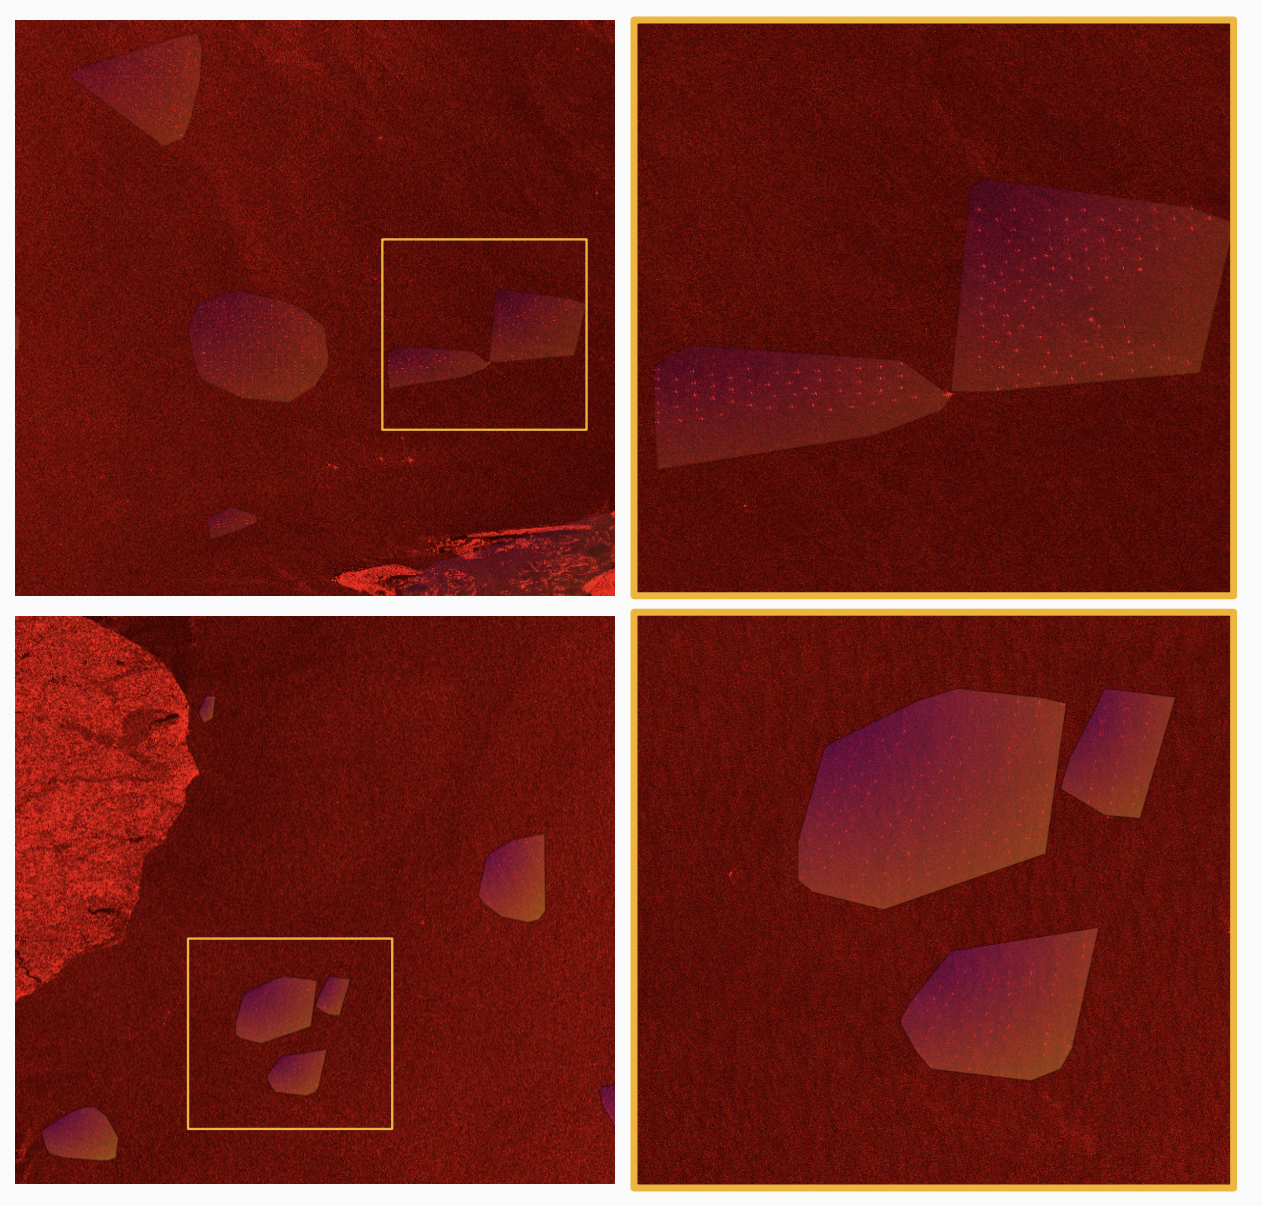
\includegraphics[width=\columnwidth]{images/good-results.png}}
\caption{Final result of our algorithm parsing west of Denmark (top) and east of England (bottom). Right images shows an enlarged view clearly showing how the clustering creates a boundary even when parks are close to each other.}
\label{good-results}
\end{center}
\end{figure}

\subsection{Exceptions}

Our model did not perform equally on every case we tested (fig. \ref{bad-results}). Coastal areas around Denmark that are periodically flooded are considered "ocean" even though beaches are clearly visible. These areas were still included in our parser which caused beaches to be labeled as windmill parks. One option of resolving this would be to expand borders or try to detect beaches separately from windmills/boats.\\

The second case in which our detection fails is when a large amount of boats are present. This is notable in parsing the Chinese coast (fig. \ref{bad-results}). When a large amount of boats are clustered in an area the clustering will label this as a park. This could be avoided by filtering based on time but since harbors are always densely packed some a thorough way of filtering might be needed.

\begin{figure}[ht]
\begin{center}
\centerline{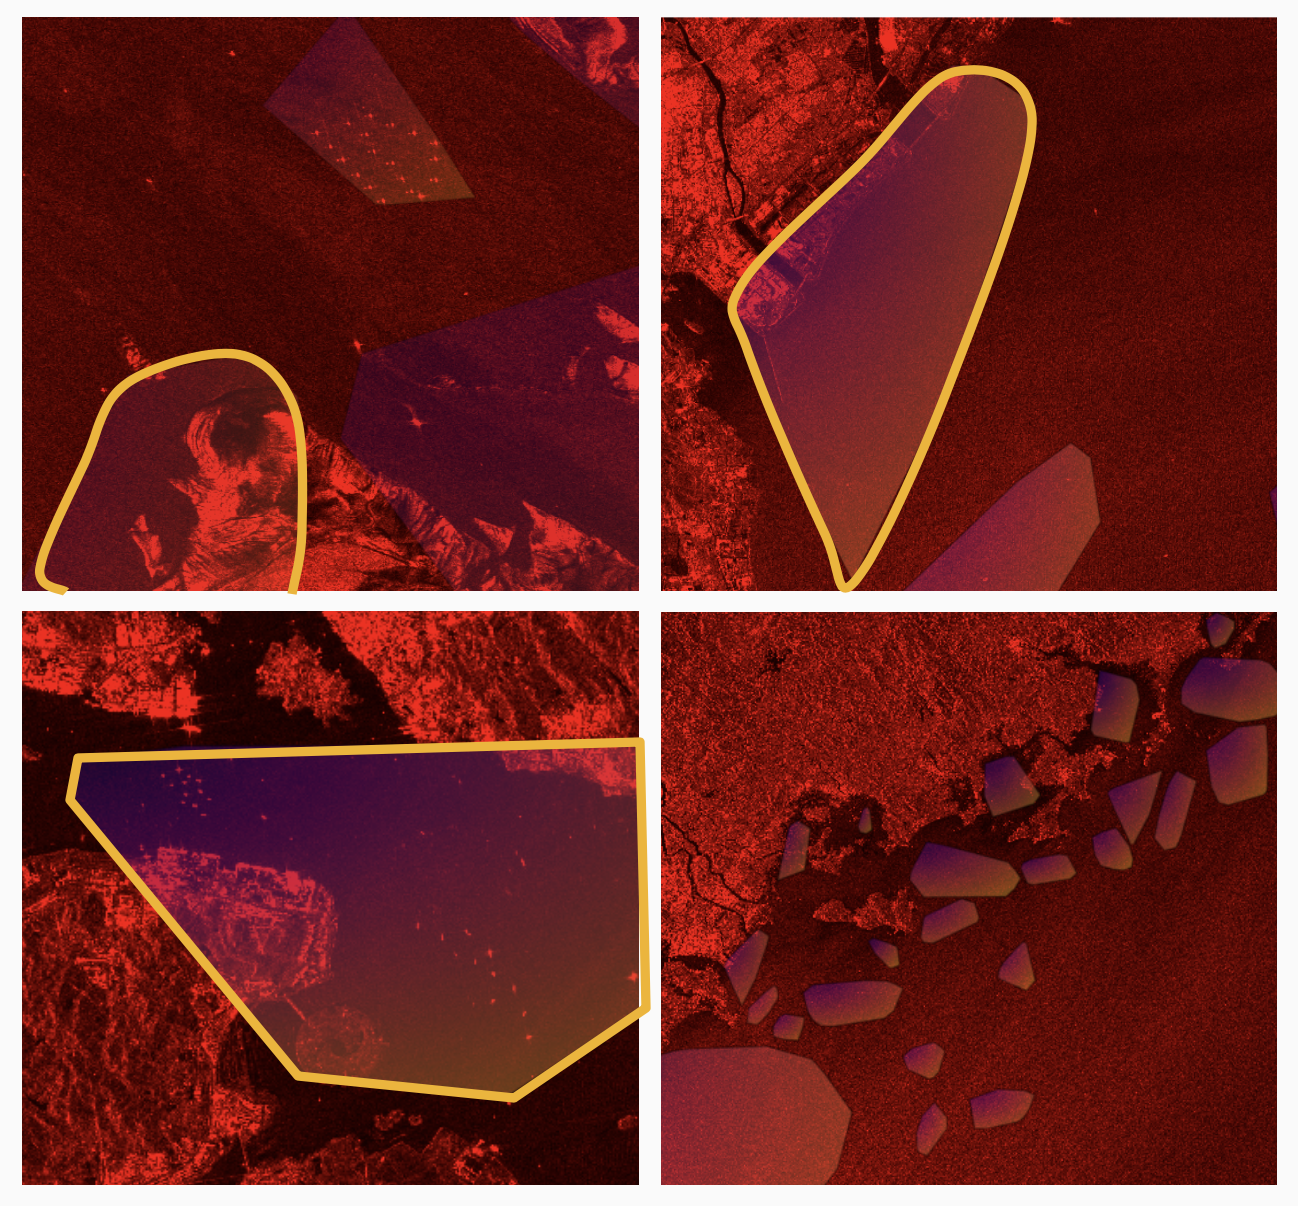
\includegraphics[width=\columnwidth]{images/bad-results.png}}
\caption{Model performing not as expected in coastal areas in Denmark (top) and harbors around China (bottom).}
\label{bad-results}
\end{center}
\end{figure}